\chapter{Pruebas\label{sec:desarrollo}}

El objetivo de este capítulo es mostrar tanto las pruebas realizadas como la metodología seguida para obtener los resultados.
Para poder entrar en detalle, en las pruebas, es necesario hacer un repaso de los dispositivos hardware y software que se encuentran disponibles. Una vez conocidos, es posible definir una metodología de pruebas, así como una descripción de las mismas en los diferentes entornos.

\lsection{Entorno de Desarrollo\label{sec:entorno}}

Escoger un entorno de desarrollo y pruebas adecuado, supone realizar multitud de comparativas y pruebas entre los diferentes elementos disponibles, tanto a nivel software, como a nivel hardware.
Poner a prueba todos y cada uno de los posibles elementos supone un reto en cuanto a coste monetario como en tiempo, y dado que tanto el presupuesto como el tiempo de realización del doble trabajo fin de máster son finitos, se ha partido del siguiente equipamiento facilitado por el grupo de investigación HPCN.

\subsection{Equipamiento de prueba utilizado\label{sec:equipamiento}}

El equipamiento de prueba utilizado costa de 3 elementos fundamentales: Captura de tráfico, emisión de tráfico y el tráfico emitido como tal.
Todos estos elementos son de vital importancia a la hora de realizar una comparativa, pues tan importante es el proceso de captura, como que los datos recibidos hayan sido emitidos correctamente. Estos datos, por otro lado, deben representar algún tráfico significativo para las pruebas, ya sea un caso extremo, o un caso realista. Cada una de estas partes es explicada con detalle a continuación:
\\
\\

\subsubsection{Equipo de captura y desarrollo}

El equipo de captura y desarrollo es conocido internamente por el nombre de \textit{Nrg}.
Esta sonda de captura, está compuesta por una arquitectura de tipo \gls{numa} con dos procesadores \textit{Intel Xeon E5-2630} a una velocidad de 2.6~Ghz cada uno.
Ambos procesadores se encuentran conectados a 2 tarjetas de memoria de 8~GB cada una, haciendo un total de 32~GB para todo el sistema.
Este equipo cuenta con diversos PCIe generación 3 que permiten transferencias de datos de hasta casi un 1~GBps por cada linea PCIe. El equipo cuenta con los siguientes dispositivos PCI:

\begin{itemize}
\item \textbf{Tarjeta gráfica Nvidia Tesla K40C}: A pesar de no haber sido utilizada la tarjeta gráfica a lo largo de las pruebas o el desarrollo, parece interesante mencionar su presencia en el bus PCIe.

\item \textbf{Tarjeta de red Ethernet Mellanox MT27500 (ConnectX-3)}: Esta tarjeta es capaz de establecer velocidades de enlace de entre 40 y 56~Gbps. Aunque inicialmente se pretendía probar esta tarjeta, Intel~\gls{dpdk} no publicó los drivers para explotar esta tarjeta hasta la versión 2.0, la cual fue publicada en abril de 2015. De igual modo, no disponemos de ningún emisor de tráfico fiable capaz de saturar este enlace, ni tampoco la capacidad de realizar el almacenamiento a disco a esta tasa de red sin realizar algún tipo de filtrado de tráfico. Hasta donde llega mi conocimiento, no existe (aparte del nuevo driver de Intel~\gls{dpdk} y el driver nativo) ninguna aplicación similar contra la que comparar resultados. Por todo esto, el uso de esta tarjeta ha sido descartado al encontrarse fuera del marco de este trabajo. Esta tarjeta conecta la máquina de captura con la máquina llamada \textit{Onelab3}.

\item \textbf{Tarjeta de red Ethernet Intel I350}: Esta tarjeta dispone de dos \glspl{nic} a 1~Gbps cada una. Dado la máquina de captura se encuentra inaccesible físicamente, se ha utilizado esta tarjeta como medio para el acceso remoto, así como el acceso a diferentes recursos y paquetes de Internet.

\item \textbf{Tarjeta de red Ethernet Intel 82599ES}: Esta tarjeta dispone de dos \glspl{nic} SFP+ a 10~Gbps cada una. El chipset \textit{82599ES} es compatible con la mayoría de capturadores de bajo coste actuales, por lo que la convierte en el dispositivo predilecto de cara a realizar una comparativa de rendimiento. Además, soporta diferentes modos de virtualización (\gls{passthough} y \gls{sriov}), permitiendo de esta forma alcanzar los objetivos planteados en este trabajo. Las dos interfaces de la tarjeta se encuentran conectadas al emisor de tráfico (llamado \textit{Dagda}), el cual será explicado más adelante.

\item \textbf{Controladora MegaRAID SAS-3 3108}: Dadas las limitaciones del chasis de la sonda de captura, la controladora RAID es capaz de gestionar hasta un máximo de 12 discos duros. Estos discos duros, pueden conformar desde un único Raid 0, hasta un conjunto de diferentes tipos de Raid. 
\end{itemize}

%seria interesante preguntar a victor por paper de referencia
Una vez observados los diferentes dispositivos disponibles, parece interesante realizar un inciso en la controladora raid.
Si bien puede gestionar hasta 12 discos duros, el precio de estos no es en absoluto despreciable.
En este caso, se parte de discos mecánicos \textit{Hitachi HUA 72303} (especiales para servidores) con 3~TB de capacidad cada uno.
El precio actual aproximado de estos discos duros oscila entorno a los \textit{310€}, elevando el coste de almacenamiento a más de \textit{3700€}.
Por este motivo, determinar cual es la cantidad de discos duros necesarios para cada escenario es de vital importancia de cara a reducir el coste de la sonda de captura.


\subsubsection{Equipo de emisión de tráfico}

Existen multitud de herramientas de emisión de tráfico.
Una de las herramientas clásicas es \href{http://tcpreplay.appneta.com/}{TCPReplay}.
Dicha herramienta parte de un fichero estándar \textit{PCAP} y lo transmite por una determinada interfaz de red. TCPReplay, proporciona cierto valor añadido, ya que puede regular la velocidad de transmisión entre otras muchas cosas. No obstante, esta herramienta al igual que la mayoría de emisores de tráfico clásicos (Como pktgen, etc), no es capaz de emitir tráfico a 10~Gbps, aun si este se encuentra en memoria. Esto se debe a que las herramientas de transmisión y generación de tráfico utilizan la pila de red completa del Kernel y los drivers \gls{vanilla} de las tarjetas de red.

De cara a solventar el problema de la generación y transmisión de tráfico, se han construido multitud de herramientas. Los generadores de tráfico software se basan en la reutilización de los drivers optimizados de captura como \gls{dpdk} o \textit{PacketShader}. No obstante, los emisores de tráfico software presentan serias limitaciones.
%
En el caso del emisor de \textit{PacketShader}~\cite{dpdk:packetshader}, se presentan ciertas irregularidades en la tasa de tráfico: emisión a ráfagas, problemas en los contenidos de los paquetes y en general problemas de estabilidad. De cara a hacer una comparativa de rendimiento y tasa de captura, estas irregularidades complicarían y harían fluctuar las medidas, por lo que este emisor fue descartado.
%
Por otro lado, Intel \gls{dpdk} proporciona una herramienta de emisión de tráfico bastante sofísticada conocida como \textit{Pktgen-\gls{dpdk}}~\cite{bib:dpdkpktgen}, la cual, poco a poco, se está convirtiendo en una conocida aplicación. 
La herramienta \textit{Pktgen} es capaz de saturar fácilmente 4 enlaces a 10~Gbps mediante tráfico sintético. Para conseguirlo, reserva las estructuras de los paquetes en memoria y las envía a cada una de las \gls{nic}. Esta herramienta, aunque útil para probar casos extremos, se ve perjudicada si lo que se desea es enviar tráfico almacenado previamente en un fichero. Debido al sobrecoste de las estructuras de los paquetes%
\footnote{Cada estructura de \gls{dpdk} almacena diversa información referente a un paquete. De cara a mantener la coalescencia de las cachés, estas estructuras cuentan con 2048 Bytes (La potencia de 2 más próxima a la \gls{mtu} de la red) para almacenar el payload del paquete.}%
 que utiliza \gls{dpdk}, no es posible almacenar más que unos pocos centenares de miles de paquetes por GigaByte. Aunque este número pueda aparentar ser muy grande, recordemos que en una red de 10~Gbps, se pueden llegar a mandar hasta casi 15 millones de paquetes por segundo (en caso de paquete mínimo), por lo que esta cantidad de paquetes representaría menos de una décima parte de segundo del tráfico del enlace.
 
En el otro lado, se encuentran los generadores hardware basados en \glspl{fpga}. Dentro del grupo de investigación HPCN ha sido desarrollado un potente y versátil generador de tráfico a 10~Gbps~\cite{zazo2014tnt10g}. Este generador, aporta un nivel de control en la transmisión de las tramas muy preciso, permitiendo simular, tanto cualquier situación de una red real, como casos extremos incluso a nivel físico.
Para lograr estas características, este sistema utiliza un formato especial de fichero denominado \textit{simple}. Este fichero es similar al formato PCAP, salvo porque almacena la cantidad de ceros que existen a nivel físico entre dos paquetes, lo que permite tener un elevado control y precisión durante la emisión. Dichos ficheros se encuentran en un Raid 0, de forma que un driver intermedio es capaz de acceder de forma eficiente a ellos y copiarlos en \glspl{huge}. Estas páginas son transferidas a la \gls{fpga} a través del bus PCIe. La \gls{fpga} emite el tráfico por una o varias de las diferentes \gls{nic} que posee. Como contrapartida, aunque la \gls{fpga} dispone de hasta 4 interfaces de 10~Gbps, solo es capaz de recibir hasta 10~Gbps por PCIe, por lo que como mucho podrá enviar el mismo tráfico simultáneamente por las diferentes \glspl{nic}. En la figura~\ref{fig:rafaDagda} se muestra un esquema del funcionamiento del generador y emisor de tráfico hardware.

\begin{figure}[!htb]
\centering
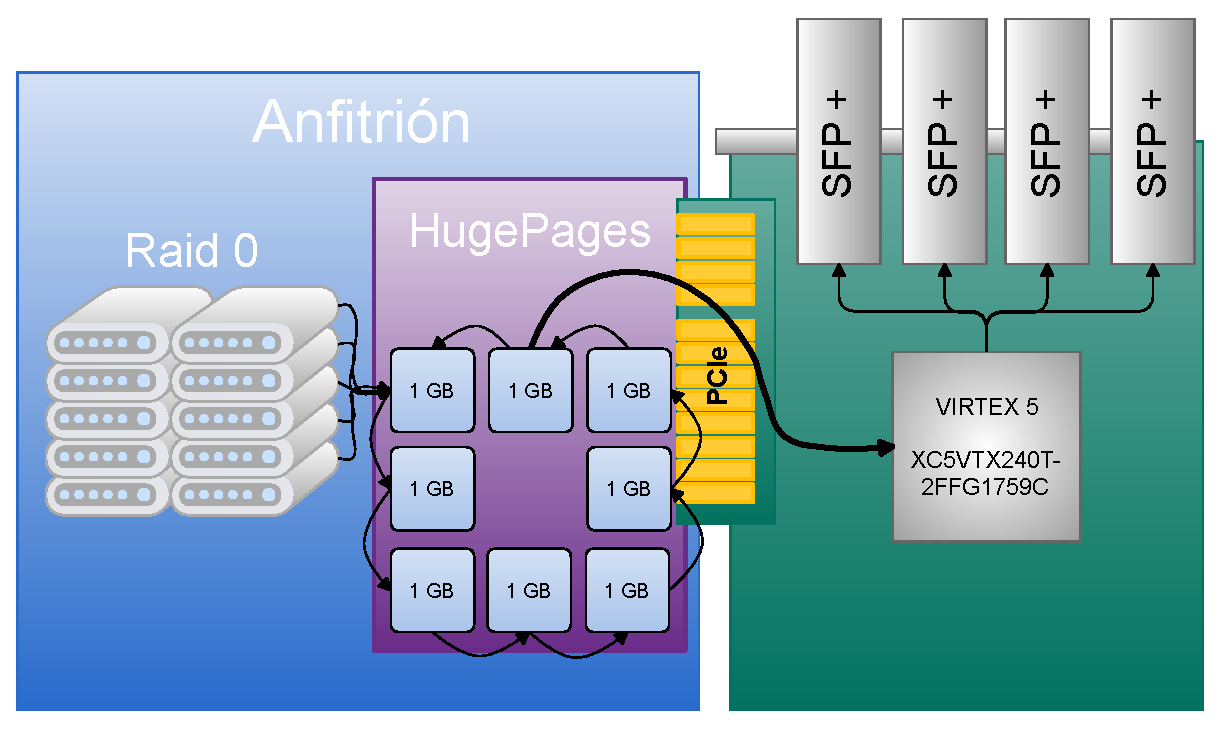
\includegraphics[scale=.6]{rafaDagda}
\caption{Arquitectura del emisor de tráfico}
\label{fig:rafaDagda}
\end{figure}

Tras escoger el generador de tráfico hardware, se definió un interconexionado de las diferentes máquinas que formarán parte de las diversas pruebas. La máquina encargada de la transmisión de tráfico (llamada \textit{Dagda}) se conecta mediante 2 interfaces de 10~Gbps a la máquina capturadora de tráfico (llamada \textit{Nrg}). La máquina de captura se encuentra a su vez conectada por un enlace de 40~Gbps con una máquina llamda \textit{Onelab3}. No obstante, y como se ha mencionado anteriormente, este enlace queda en desuso debido a la falta de software necesario para explotarlo adecuadamente. En la figura~\ref{fig:conexiones} se muestra gráficamente este interconexionado.

\begin{figure}[!htb]
\centering
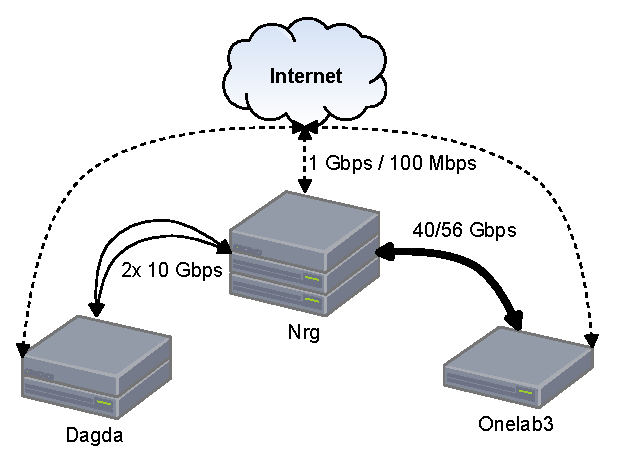
\includegraphics[scale=.8]{conexiones}
\caption{Conexionado del equipo de captura y desarrollo}
\label{fig:conexiones}
\end{figure}

\subsubsection{Tráfico emitido}

Una vez se ha decidido tanto el funcionamiento de la sonda de captura, como el hardware que se utilizará, es necesario definir el tráfico con el que se realizarán las evaluaciones, pruebas y comparativas. Para poder tener medidas útiles, es necesario poner al equipo de captura al límite, forzando y poniendo el sistema en el peor caso posible. No obstante, como se comentó en la introducción, resulta complicado encontrar enlaces completamente saturados, por lo que resulta interesante contar con tráfico representativo real.

Con el objetivo de cubrir ambos escenarios, se han utilizado los siguientes tipos de tráfico:

\begin{enumerate}

\item \textbf{Tráfico extremo}: Dentro del protocolo Ethernet, existen dos casos peores posibles: Un enlace en la que solo hay paquetes de 64 bytes y supone una tasa de 14.88 Millones de paquetes por segundo, o un enlace, en la que solo hay paquetes de tamaño 1500 y unos 800 mil paquetes por segundo.
En el primer caso, tan solo un 76\% de los bytes transmitidos%
\footnote{Los paquetes Ethernet tienen diversos campos, como el interframe gap o el preludio, que deben ser transmitidos pero no aportan ninguna información relevante. Por este motivo, dichos campos nunca son transmitidos por la tarjeta hacia el ordenador anfitrión y no pueden ser almacenados. En caso de que los paquetes sean muy pequeños, estos bytes ``ocultos'' se hacen relevantes.} %
 en el enlace son almacenados, mientras que en el segundo caso se almacenan entorno al 98\% de los bytes. Mientras que el primer caso requiere una mayor necesidad de computo para procesar un gigantesco número de paquetes, el segundo caso requiere de una mayor capacidad de escritura a disco.
Las herramientas proporcionadas por el generador de tráfico hardware escogido, son capaces de generar ambos escenarios extremos sin la necesidad de construir una traza a medida para la prueba.

\item \textbf{Tráfico Real}: Para poder obtener a tráfico real representativo a alta velocidad, es necesario recurrir a redes de grandes empresas o grandes nodos de interconexión de algún \gls{isp}. Esto causa, que la naturaleza de este tipo de tráfico suela ser confidencial o deba mantener ciertos requisitos de privacidad, por lo que, es complejo acceder a este tipo de muestras de tráfico.
Dentro de este contexto, la organización \href{http://www.caida.org/home/}{Caida}, captura tráfico en nodos que interconectan grandes ciudades de Estados Unidos. Tras realizar un proceso de anonimización\footnote{El proceso de anonimización consiste en truncar los paquetes eliminando la capa de aplicación.}, la organización Caida publica estas capturas de tráfico para su posterior uso por investigadores. Dentro de las trazas disponibles, se ha escogido una muestra unos 7 minutos de duración entre la ciudad de Seattle y la ciudad de Chicago el día 1 de octubre de 2014~\cite{caida2014}. Aunque esta traza está capturada en un enlace a 10~Gbps, la velocidad efectiva del tráfico ronda los 5~Gbps con un tamaño medio de paquete de unos 965 Bytes. De cara a realizar las pruebas y estresar un poco el sistema, se ha decidido acelerar transmisión de esta traza, reduciendo el tiempo entre los paquetes al mínimo posible.

\end{enumerate}

\subsection{Software utilizado\label{sec:sw}}

Encontrar el software apropiado para realizar un desarrollo es una tarea tediosa. Dado que el objetivo de este trabajo fin de máster es la realización de un motor de captura y almacenamiento de tráfico con Intel~\gls{dpdk} y la realización de una comparativa entre los diferentes métodos de captura en diferentes entornos de ejecución, es necesario plantear un entorno software aceptable para un posible cliente.
%
En el mundo empresarial, predomina el uso de las distribuciones de linux basadas en red hat o en suse. No obstante, la tecnología de virtualización, requiere de los últimos avances para poder ser explotada al máximo. Con esto en mente, la distribución de linux que mejor cumple estas condiciones es Fedora. Por este motivo, en la sonde captura se ha instalado un Fedora 20.

La mayoría de los entornos de virtualización de los que disponen las grandes compañías son: \gls{kvm}~\cite{bib:kvm}, XEN~\cite{bib:xen} o la versión profesional de VMWare~\cite{bib:vmware}. De cara a un presupuesto limitado, descartamos la opción de utilizar VMWare desde el principio. La decisión entre los hypervisores \gls{kvm} y XEN es algo más compleja pues son ambos sistemas muy utilizados, ambos son gratuitos y ambos se encuentran en auge. No obstante, se aprecia a la comunidad investigadora más enfocada en el entorno de \gls{kvm}, así como una gran cantidad de esfuerzo por parte de la comunidad de \gls{kvm} en el desarrollo de elementos y técnicas avanzadas de virtualización como \gls{virtio}. Por estos motivos, se ha escogido \gls{kvm} como método de virtualización.
%
Como optimización, dado que varios de los motores de captura hacen uso de las \glspl{huge}, se ha configurado el sistema de virtualización \gls{kvm} para que reserve la memoria de las máquinas virtuales en \gls{huge} con el objetivo de que el rendimiento en las \glspl{vm} no se vea excesivamente afectado por problemas de paginación o problemas de cache~\cite{kudryastev2013pcs}. Las máquinas virtuales, a su vez, proveen \gls{huge} a los diferentes motores que se ejecutan en ellas.
%
Cada una de las máquinas virtuales utilizadas está formada por 3 \glspl{core} virtuales, mapeados y reservados en 3 \glspl{core} físicos. Cada máquina virtual cuenta a su vez con 5~GB de memoria RAM.

Una vez que tenemos los más pilares básicos de nuestro sistema de captura, es necesario hacer un pequeño énfasis en lo que a funciones virtuales se refiere. Tal y como se ha explicado en capítulos anteriores, las funciones virtuales son a todos los efectos un dispositivo PCIe más. No obstante, las tarjetas Intel ofrecen diversas formas de crear y gestionar sus \glspl{nfv}. Por un lado, el driver \gls{vanilla} \textit{ixgbe}, permite indicar a la tarjeta que cree un número determinado de \glspl{nfv}, de una forma muy sencilla. No obstante, este tipo de funcionamiento delega todo el control de la función virtual a la tarjeta física, sin que la CPU intervenga en ningún caso en el trasiego de paquetes.
%
Por otro lado, el driver proporcionado por \gls{dpdk}, proporciona su propia forma de gestionar las funciones virtuales. Este paradigma, rompe ligeramente el concepto de \gls{vf}, ya que \gls{dpdk} requiere del uso de un determinado programa, llamado \textit{testpmd}, que de forma activa ayuda a la tarjeta a manejar las diferentes funciones virtuales. No obstante, este método obliga a la \gls{cpu} a trabajar, consumiendo, como mínimo, un \gls{core} completo. De cara a evaluar que método es el mejor, se han tenido en cuenta ambas aproximaciones y se detallan los resultados de la comparativa en la sección~\ref{sec:sriov}.

Dentro del software de captura de tráfico se ha decidido realizar una comparativa entre los siguientes motores: \gls{dpdk}, \textit{HPCAP}, \textit{PF\_RING}, y el driver \gls{vanilla} \textit{ixgbe} mediante el programa de captura simple basado en \textit{libPCAP}~\cite{bib:tcpdump}.%\textit{TCPDump}~\cite{bib:tcpdump}. 
El resto de motores de captura han sido descartados para las pruebas, dado que su funcionamiento es muy similar entre sí, y ninguno de ellos es capaz de operar con~\gls{nfv}. Los motores de captura han sido explicados previamente en el capítulo~\ref{sec:estado_del_arte}.

\lsection{Metodología de las pruebas\label{sec:metod}}

Realizar todas y cada una de las pruebas que se describen en las siguientes secciones, supone un trabajo tedioso y en un principio muy manual. Si bien son importantes los resultados de las pruebas, es de igual importancia mantener un cierto protocolo a la hora de realizarlas asegurando su repetibilidad así como almacenar los resultados de forma organizada. 
Para llevar esto a cabo, se realizó un documento interno que incluían los pasos a la hora de lanzar una prueba en los diferentes escenarios, así como los parámetros recomendados para cada una de las diferentes aplicaciones.

Cada una de las aplicaciones de captura tiene su propia forma de representar las diferentes estadísticas relacionadas con la \gls{nic} que está utilizando para capturar (como paquetes recibidos, paquetes perdidos, paquetes con errores, etc).
De cara a normalizar estos datos, se realizaron diferentes scripts encargados de interpretar la salida de cada una de las aplicaciones y convertirlas a un formato único. El formato planteado se basa en un simple fichero de texto de 4 columnas separadas por tabulaciones. Cada línea de este fichero, representa un determinado instante de tiempo en el que se consultaron las estadísticas de una única \gls{nic}. En caso de que la aplicación esté gestionando más de una interfaz de red, se generan tantos ficheros como \glspl{nic} utilice.

El fichero de estadísticas de una \gls{nic} consta de las siguientes columnas:

\begin{enumerate}
\item Momento en formato unix en el que se realizó la medida.
\item Velocidad en Gigabits por segundo entre el momento anterior y el actual.
\item Paquetes recibidos entre el momento anterior y el actual.
\item Paquetes perdidos entre el momento anterior y el actual.
\end{enumerate}

Para poder mantener una organización entre las diferentes pruebas, estos ficheros son almacenados en un árbol de carpetas. Este árbol se subdivide en nombre de la prueba, tráfico utilizado, motor de captura utilizado y marca temporal del inicio de la prueba.
Dado que estos ficheros representan una serie temporal, que aporta cierta información de depuración, se ha realizado un nuevo script que resume los diferentes ficheros asociados a cada prueba, generándose así un pequeño informe de resultados de cada una de las pruebas realizadas.

La complejidad de los capturadores de tráfico es elevada. Por ello, estas aplicaciones cuentan con multitud de parámetros que los permiten acomodarse a diversos entornos. Estos parámetros engloban desde el \gls{core} en el que se ejecuta un determinado componente del capturador, hasta el tamaño de los descriptores de paquete o la longitud de las colas de recepción.
%
Para que la comparativa entre los diferentes motores de captura sea justa, es necesario repetir multitud de veces determinadas pruebas en busca de los parámetros adecuados. Del mismo modo, es necesario que todas las pruebas se ejecuten en las mismas condiciones, evitando fluctuaciones debido a otros efectos colaterales de haber ejecutado anteriormente una prueba con otro capturador (como elementos cacheados o cambios colaterales en el funcionamiento de algún dispositivo). Por este motivo, se desarrollaron dos protocolos de realización de pruebas, una para entornos físicos y virtuales mediante \gls{passthough} y otro para entornos virtuales con \glspl{nfv}:

\begin{itemize}
\item \textbf{Procedimiento en entorno físico y virtual con \gls{passthough}:}
\begin{enumerate}
\item Se reinicia la máquina (física o virtual) con la configuración adecuada (\glspl{huge} si son necesarias, etc).
\item Se resetea el generador de tráfico.
\item Se instancia el driver y programa de captura.
\item Se inicia la transmisión de tráfico por parte del generador.
\item Al terminar la ejecución del programa de transmisión, se cierra el programa de captura y se almacenan los resultados.
\end{enumerate}

\item \textbf{Procedimiento en entorno virtual con \gls{nfv}:}
\begin{enumerate}
\item Se instancia el driver encargado de la generación de \gls{nfv} y se configura.
\item Se reinicia la máquina virtual con la configuración adecuada a la prueba.
\item (Si procede) se inicia el programa \textit{testpmd} de Intel~\gls{dpdk} en el anfitrión.
\item Se resetea el generador de tráfico.
\item Se instancia el driver en la máquina virtual y programa de captura.
\item (Si procede) se configura el programa \textit{testpmd}.
\item Se inicia la transmisión de tráfico por parte del generador.
\item Al terminar la ejecución del programa de transmisión, se cierra el programa de captura y se almacenan las estadísticas tanto de la máquina virtual como de la máquina física.
\end{enumerate}

\end{itemize}

\lsection{Pruebas en entorno físico\label{sec:fisico}}

El régimen clásico de funcionamiento de las múltiples herramientas de red es el entorno nativo o físico. Dado que estas herramientas usualmente requieren de una gran cantidad de procesamiento así como de ancho de banda en la memoria para funcionar a altas (e incluso no tan altas) velocidades, hasta hace poco era impensable llevar a estas herramientas a un entorno virtual, salvo para realizar tareas con muy poca cantidad de datos.
Por este motivo, el entorno físico es el punto de partida en la realización de cualquier comparativa de herramientas de red, lo que incluye a los capturadores de red.

La arquitectura del entorno físico es simple. Una tarjeta de red y una controladora Raid, mediante sus correspondientes drivers, se conectan a un motor de captura. De esta forma, el trabajo del motor de captura se resume en una copia de los datos que llegan desde la red hasta el Raid de alta velocidad. En un principio, esta tarjeta de red, se encontraría conectada a un switch o a un router de la red que deseamos monitorizar, el cual, nos duplica todo el tráfico que circula por la misma mediante un puerto de SPAN. Dado que en este caso, no se ha podido acceder a una red de alta velocidad, se ha simulado este enlace mediante el generador hardware comentado previamente.

Si el servidor de captura es suficientemente potente, es posible que en paralelo se encuentren en ejecución otras aplicaciones en nuestra sonda de captura. Estas aplicaciones pueden encargarse de leer los datos almacenados en el Raid y sacar algún tipo de análisis, o incluso, ejecutar algún tipo de servicio que no esté directamente relacionado con la captura como un servidor web o una máquina virtual completa. Esta arquitectura puede verse en la figura~\ref{fig:vmfisica}.

\begin{figure}[!htb]
\centering
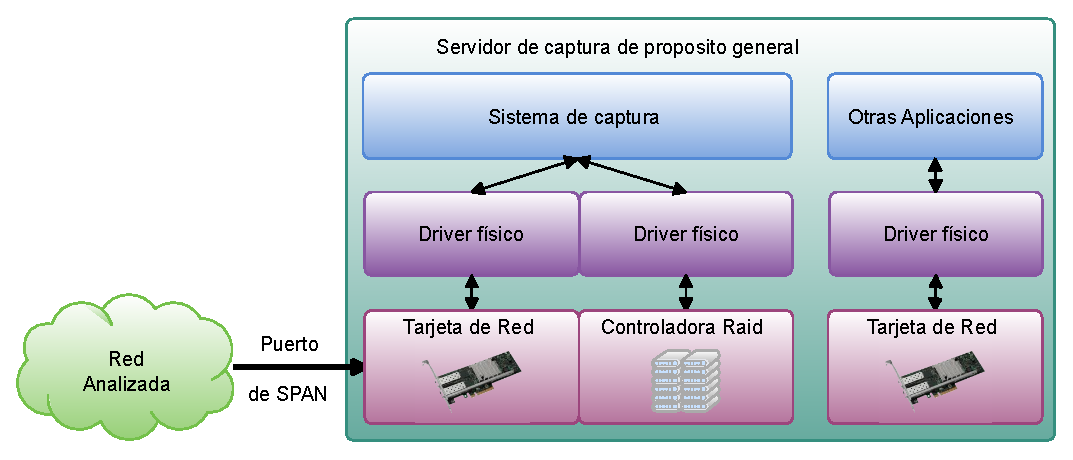
\includegraphics[scale=.6]{VMfisica}
\caption{Arquitectura de captura clásica}
\label{fig:vmfisica}
\end{figure}

Un sistema de captura y almacenado, como su nombre indica, se divide en dos partes: captura y almacenado. Ambos sistemas utilizan y explotan al máximo el ancho de banda de la memoria y el ancho de banda de los diferentes buses de comunicaciones. Por ello, es necesario realizar una comparativa que mida el caso mejor de ambos procesos por separado.

De cara a hacer una prueba de rendimiento del sistema de almacenado (Raid 0), se ha reutilizado un script que permite, dinámicamente, cambiar el número de discos que conforman el Raid de captura. Ya que los motores de captura de los que se dispone, almacenan sucesivos ficheros de 2~GB, este script se encarga también de realizar sucesivas escrituras de ficheros de 2~GB mediante la herramienta de \textit{GNU}, \textit{dd}. Tal y como se ha comentado anteriormente, para poder escribir a esta velocidad en un raid es necesario saltarse las copias intermedias que realiza de forma natural el kernel de \textit{Linux}. Para lograrlo, existe el modo de escritura \textit{Direct}, que permite al kernel copiar directamente desde la memoria del usuario a nuestro raid de captura.


\begin{figure}[!htb]
\centering
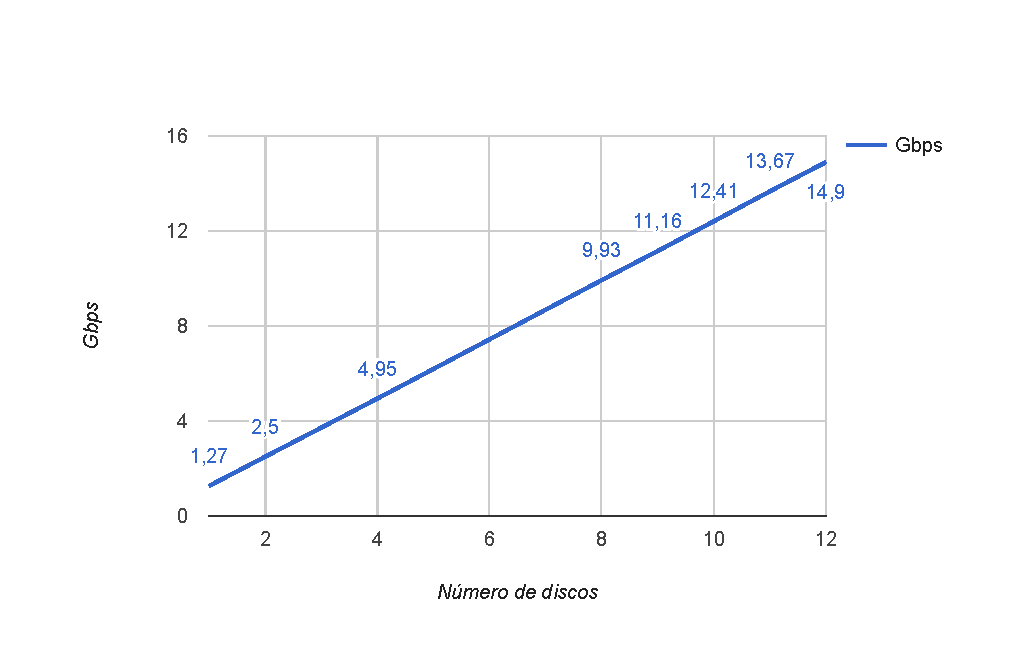
\includegraphics[scale=.7]{graph1}
\caption{Rendimiento de escritura en Raid 0 sin virtualización}
\label{fig:vmfisica:graphdd}
\end{figure}

Tal y como puede observarse en la figura~\ref{fig:vmfisica:graphdd}, la tasa de escritura a disco parece crecer de forma lineal con el número de discos que conforman el raid. A raíz de estos resultados, parece viable crear un raid de tan solo 9 discos para las pruebas, pues en media ofrece una tasa de escritura de más de los 10~Gbps a los que se recibe el tráfico. No obstante, y para mayor seguridad, se han realizado varios cientos de prueba de escritura para poder obtener un intervalo de confianza del rendimiento que proporciona el Raid con 9 discos. Dicho intervalo se encuentra entre 11,09 y 11,23~Gbps, lo que nos asegura en cierta medida que el rendimiento será suficiente para almacenar todo el tráfico.

Una vez se ha medido el rendimiento del raid de almacenamiento el caso óptimo, es posible comenzar a realizar las primeras pruebas de captura con los diferentes motores.
Dado que en esta primera prueba, se busca encontrar las limitaciones de los capturadores de tráfico, se han utilizado unas pequeñas aplicaciones que tan solo reciben el tráfico y no realizan ningún procesado sobre los mismos. Mientras que los motores \textit{HPCAP} y \textit{PF\_RING} proporcionan sus propias herramientas básicas de testeo, se ha realizado una herramienta propia en \gls{dpdk} para realizar este tipo de mediciones. De igual modo, se ha reutilizado una pequeña aplicación realizada en \textit{libpcap} para probar la tasa de captura del driver \gls{vanilla} \textit{ixgbe}.

Los resultados de esta primera prueba, pueden observarse en la tabla~\ref{tab:vmfisica:soloCap}. Estos resultados, resultan en cierta medida sorprendentes pues el driver \gls{vanilla} de Intel ha mejorado en gran medida con los años, pudiendo incluso capturar 10~Gbps sin perdidas cuando se enfrenta a un tráfico realista.
También cabe destacar, el rendimiento del motor de captura \textit{PF\_RING}. A pesar de obtener un buen rendimiento al enfrentarse a una única \gls{nic}, el rendimiento decrece y comienza perder paquetes cuando debe enfrentarse a 2 interfaces de red simultáneamente.
El rendimiento de \textit{HPCAP}, parece bastante razonable si recordamos su filosfía de \gls{onecopy}. Finalmente, en esta tabla se puede observar como la tecnología de captura más novedosa sale ganando en esta prueba sin llegar a perder ni un solo paquete en ninguna de los casos.

\begin{table}[htb]
\centering
\begin{tabular}{|c|c|c|c|c|}
	\hline
		\multirow{3}{*}{\begin{tabular}[c]{c}{\bf Motor}\\ {\bf de captura}\end{tabular}} & \multicolumn{4}{c|}{{\bf \% de paquetes procesados}}\\
	\cline{2-5}
		 & \multicolumn{2}{c|}{{\bf 1 \gls{nic}}} & \multicolumn{2}{c|}{{\bf 2 \glspl{nic}}} \\
	\cline{2-5}
		 & {\bf 64 Bytes }   & {\bf CAIDA}  & {\bf 64 Bytes}   & {\bf CAIDA}  \\ \hline
		ixgbe         & 2.7   & 100  & 3.7     & 93.55  \\ \hline
		PF\_RING      & 100   & 100  & 76.1    & 100    \\ \hline
		HPCAP         & 97.9  & 100 & 97.8  & 100     \\ \hline
		DPDK          & 100   & 100  & 100     & 100  \\ \hline
\end{tabular}
\caption{Porcentaje de paquetes capturados en un escenario sin virtualización ni almacenamiento de paquetes.}
\label{tab:vmfisica:soloCap}
\end{table}

Una vez se han obtenido los resultados de las primeras pruebas, es posible comenzar a realizar las pruebas conjuntas de captura y almacenamiento a disco. Cabe recordar, que en estas pruebas pueden empezar a surgir cuellos de botella en los accesos a memoria, así como en los accesos a los buses PCIe. Tal y como se muestra en la tabla~\ref{tab:vmfisica:CapAlmac}, el rendimiento con respecto a la tabla~\ref{tab:vmfisica:soloCap} decrece en cierta medida. Un detalle a tener en cuenta es el descenso en el rendimiento de la aplicación desarrollada en \gls{dpdk}. Al igual que el \gls{zerocopy} ayuda a mejorar el rendimiento, si el pipeline de proceso tiene demasiada latencia, se comienza a perder paquetes. Por otro lado, en una filosofía \gls{onecopy}, como la de \textit{HPCAP}, se independiza mucho mejor el procesamiento sobre los paquetes (en este caso copia a disco) del proceso de captura.
Por este motivo, la tasa de paquetes capturados utilizando \textit{HPCAP} se ve muy poco afectada cuando se añade el proceso de almacenado. Mientras que en la implementación de captura sobre \gls{dpdk}, se pierde más de un 4\% de los paquetes, frente a la implementación de solo captura que no perdía ningún paquete.
Finalmente, cabe mencionar que las pruebas sobre captura y almacenamiento se han realizado utilizando una única \gls{nic}. Dado que las pruebas del raid indican que solo es capaz de almacenar hasta 10~Gbps, carece de sentido realizar una prueba que claramente va a estar acotada por esta cifra.

\begin{table}[htb]
\centering
\begin{tabular}{|c|c|c|}
	\hline
		\multirow{2}{*}{\begin{tabular}[c]{c}{\bf Motor}\\ {\bf de captura}\end{tabular}} & \multicolumn{2}{c|}{{\bf \% de paquetes procesados}}\\
	\cline{2-3}
		 & {\bf 64 Bytes }   & {\bf CAIDA}    \\ \hline
		ixgbe         & 10,3  & 91.9     \\ \hline
		HPCAP         & 95.7  & 100     \\ \hline
		DPDK          & 95.8  & 100    \\ \hline
\end{tabular}
\caption{Porcentaje de paquetes capturados con almacenamiento y sin virtualización.}
\label{tab:vmfisica:CapAlmac}
\end{table}

%%%%%%%%%%%%%%%%%%%%%%%%%%%%%%%%%%%
\lsection{Pruebas en entornos virtuales\label{sec:virtual}}

Una vez se dispone de los primeros resultados en los entornos físicos es posible iniciar con las pruebas dentro de diferentes entornos y configuraciones virtuales.
Es fácil suponer que los nuevos resultados que se obtendrán dentro de un entorno virtualizado, sufrirán algún tipo de degradación pues inevitablemente existe una pequeña sobrecarga en el sistema debido a la ejecución simultanea de diversos sistemas operativos.

Llegados a este punto, es interesante recordar la motivación de la virtualización. La virtualización en redes de comunicaciones suele venir por temas de escalabildiad, o problemas a la hora de insertar una nueva máquina en un \gls{cpd}. Esto significa, que en un principio la máquina virtual dedicada captura, va a compartir con una alta probabilidad la maquina física en la que se encuentra. Esto hace plantearse diferentes métodos para compartir los recursos y operar dentro de estas \glspl{vm}. Por ello, en esta sección se pretende mostrar, no solo las diferentes combinaciones de virtualización de los dispositivos, sino también, una comparativa en cuanto ventajas y desventajas que suponen cada uno de estos métodos.

\subsection{Usando Paravirtualización: VIRTIO\label{sec:virtio}}

Antes de que los sistemas de virtualización contasen con la tecnología necesaria para realizar \gls{passthough} o \gls{sriov}, se recurría a la virtualización completa del dispositivo y a la paravirtualización. Dado que el objetivo es alcanzar altas tasas de captura y almacenamiento, puede parecer poco producente dedicar esfuerzo a probar esta clase de tecnología que requiere un gran esfuerzo por parte del hypervisor a la hora de realizar el interconexionado entre el mundo físico y el mundo virtual.

Dado que existe un gran esfuerzo en optimizar el sistema de paravirtualización de \gls{kvm} con los módulos \gls{virtio}, se ha decidido darle una oportunidad. A diferencia de un sistema de virtualziación completo, una paravirtualización construye un pequeño hardware virtual que permite compartir un determinado dispostivo hardware entre la máquina física y diversas máquinas virtuales. Este pequeño hardware virtual, es lo suficientemente ligero como para no suponer una elevada perdida de rendimiento pero lo suficientemente completo como para proporcionar, en principio, todas las funcionalidades del hardware original. Este hardware virtual, requiere a su vez de drivers especiales en las máquinas virtuales.

Teniendo en cuenta que los dispositivos \gls{virtio} se construyen como una aplicación más que utiliza el hardware subyacente, parece que la aproximación de utilizar \gls{virtio} con la tarjeta de red, pierde sentido. Si bien, el driver \textit{ixgbe} es incapaz de ofrecer un rendimiento consistente e independiente del procesamiento, añadir una nueva capa de procesamiento solo empeorará el rendimiento. Por este motivo, se ha descartado utilizar \gls{virtio} con las tarjetas de red.

Por otro lado, la idea de poder compartir un raid entre diferentes máquinas virtuales parece atractiva. No obstante, resulta complicado encontrar tarjetas Raid con soporte \textit{sriov}, y las que lo soportan no suelen ser capaces de asociar un raid a más de una función virtual, impidiendo así su compartición. Por otro lado, los driver \gls{virtio} permiten compartir un cualquier dispositivo de bloques entre diferentes máquinas virtuales. Es importante mencionar, que dado que este tipo de compartición se hace a nivel de dispositivo de bloques, si varias máquinas virtuales escriben a la vez sobre un sistema de ficheros, pueden llegar a darse problemas e incluso a corromperse el sistema de ficheros perdiendo toda la información del Raid. A pesar de este riesgo, este modelo sigue resultando atractivo en temas de monitorización, en donde una máquina virtual escribe a disco los datos de red y otras máquinas virtuales los leen únicamente para realizar diferentes tipos de análisis.
%
Para analizar el rendimiento de los driver \gls{virtio} se ha realizado el mismo conjunto de pruebas de escritura en el raid que en la sección anterior cuyos resultados pueden observarse en la figura~\ref{fig:vmfisica:graphdd2}.
Si miramos con detalle los resultados obtenidos, podremos observar que el rendimiento del raid no ha caído, sino que ha aumentado muy ligeramente con respecto a la versión física. Aunque pueda parecer extraño, esto es debido al funcionamiento de \gls{virtio}. Para suplir la sobrecarga de un minidriver, \gls{virtio} se asegura de realizar las escrituras en bloques de tamaños óptimos, buffereando las diferentes peticiones de escritura. Por este motivo, y de forma extraordinaria, las escrituras a disco mediante \gls{virtio} aparentan ser ligeramente más eficientes.

\begin{figure}[!htb]
\centering
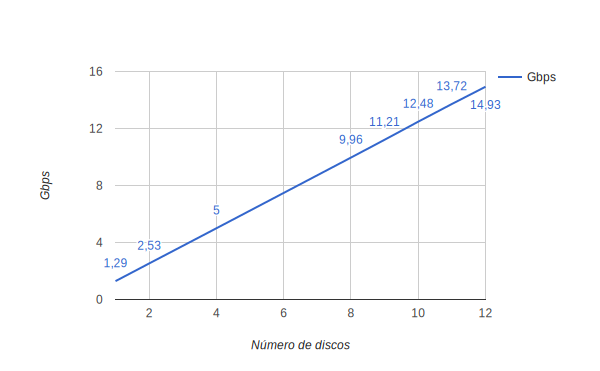
\includegraphics[scale=.7]{graph2}
\caption{Rendimiento de escritura en Raid 0 utilizando VirtIO}
\label{fig:vmfisica:graphdd2}
\end{figure}

\newpage
\subsection{Usando Passthrough\label{sec:pt}}

Dentro de los modelos de virtualización clásicos, nos encontramos con el modelo de \gls{passthough}. Este sistema de virtualización consiste en transferir todo el control sobre un determinado dispositivo a la máquina virtual. De esta forma, una \gls{vm}, es capaz de utilizar los driver nativos para susodicho dispositivo mitigando enormemente los efectos de la virtualización.

A pesar de que en términos de rendimiento la tecnología de \gls{passthough} se encuentra aventajada, esta forma de virtualización no permite que los recursos se compartan. Recordemos que una de las premisas de la virtualización es la compartición de recursos, ya que se asume que una única máquina virtual usualmente no explota al 100\% todos los recursos de los que dispone. En la figura~\ref{fig:vmpass} se muestra una arquitectura en la cual existen diversas máquinas virtuales. No obstante, aunque las aplicaciones dentro de una máquina virtual pueden compartir el harware, las aplicaciones de otras \glspl{vm} requieren sus propios dispositivos.

\begin{figure}[!htb]
\centering
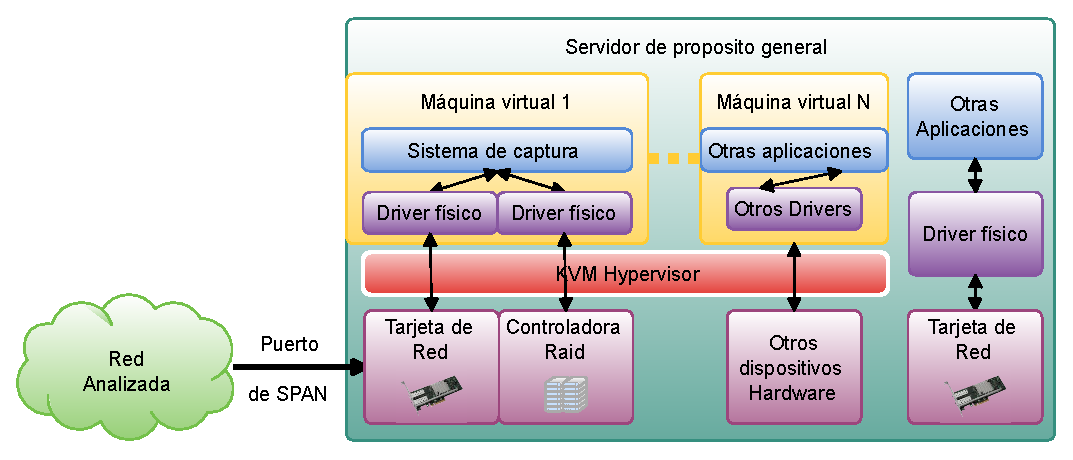
\includegraphics[scale=.6]{VMPass}
\caption{Arquitectura de captura en un escenario con Passthrough} 
\label{fig:vmpass}
\end{figure}

Bajo este paradigma de virtualización, se han vuelto a repetir las pruebas de escritura en el raid. Dado que la máquina virtual gestiona la controladora raid de la misma forma que lo haría una máquina real, el rendimiento se ve muy poco alterado con el rendimiento medido en un entorno real. Los resultados de estas pruebas pueden verse en la figura~\ref{fig:vmfisica:graphdd3}.

\begin{figure}[!htb]
\centering
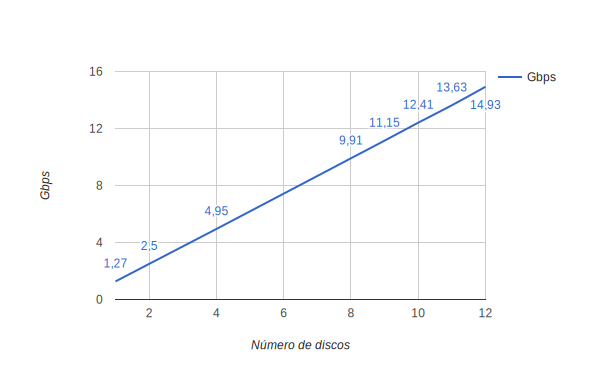
\includegraphics[scale=.7]{graph3}
\caption{Rendimiento de escritura en Raid 0 utilizando Passthrough}
\label{fig:vmfisica:graphdd3}
\end{figure}

Una de las ventajas que aportan las tarjetas de red de 10~Gbps de Intel es la representación de cada \gls{nic} como un dispositivo PCIe independiente. Esto permite que cada interfaz de la tarjeta de red pueda ser utilizada por una máquina diferente, ya sea esta física o virtual. Con el objetivo de observar como afecta dividir el tráfico entre un entorno físico y un entorno virtual, se han realizado pruebas en las siguientes 3 arquitecturas: 1 \gls{nic} en una única máquina virtual, 2 \glspl{nic} en una única máquina virtual y 2 \glspl{nic} (1+1) repartidas entre una máquina virtual y su sistema operativo anfitrión. Los resultados de la prueba de solo captura pueden verse en la taba~\ref{tab:vmpass:soloCap}.

\begin{table}[htb]
\centering
\begin{tabular}{|c|c|c|c|c|c|c|}
	\hline
		\multirow{3}{*}{\begin{tabular}[c]{c}{\bf Motor}\\ {\bf de captura}\end{tabular}} & \multicolumn{6}{c|}{{\bf \% de paquetes procesados}}\\
	\cline{2-7}
		 & \multicolumn{2}{c|}{{\bf 1 \gls{nic}}} & \multicolumn{2}{c|}{{\bf 2 \glspl{nic}}} & \multicolumn{2}{c|}{{\bf 1+1 \glspl{nic}}} \\
	\cline{2-7}
		 & {\bf 64 Bytes }   & {\bf CAIDA}  & {\bf 64 Bytes}   & {\bf CAIDA} & {\bf 64 Bytes}   & {\bf CAIDA}  \\ \hline
		ixgbe         & 1.9   & 62.7    & 2.5   & 41.8     & 6.2   & 83.7   \\ \hline
		PF\_RING      & 99.8  & 100     & 75.2  & 100      & 99.7  & 100    \\ \hline
		HPCAP         & 85.2  & 100     & 33.6  & 99.9     & 89.9  & 100    \\ \hline
		DPDK          & 100   & 100     & 100   & 100      & 100   & 100    \\ \hline
\end{tabular}
\caption{Porcentaje de paquetes capturados mediante Passthrough sin almacenamiento de paquetes.}
\label{tab:vmpass:soloCap}
\end{table}

En los resultados mostrados por la tabla anterior, se aprecia una pequeña degradación en el rendimiento cuando una única máquina virtual gestiona más de 1 \gls{nic}. Es probable que este efecto se deba a que cada una de las \glspl{vm} tiene un número de recursos limitado inferior al del sistema operativo anfitrión. Si los motores de captura requieren más recursos (ya sean \glspl{core} o memoria) y no disponen de ellos, inevitablemente el rendimiento se ve afectado.

\begin{table}[htb]
\centering
\begin{tabular}{|c|c|c|c|c|}
	\hline
		\multirow{3}{*}{\begin{tabular}[c]{c}{\bf Motor}\\ {\bf de captura}\end{tabular}} & \multicolumn{4}{c|}{{\bf \% de paquetes procesados}}\\
	\cline{2-5}
		 & \multicolumn{2}{c|}{{\bf Raid en Passthrough}} & \multicolumn{2}{c|}{{\bf Raid en VirtIO}} \\
	\cline{2-5}
		 & {\bf 64 Bytes }   & {\bf CAIDA}  & {\bf 64 Bytes}   & {\bf CAIDA}  \\ \hline
		HPCAP         & 82.2  & 100    & 82.8    & 100     \\ \hline
		DPDK          & 97.6  & 100    & 95.3    & 100  \\ \hline
\end{tabular}
\caption{Porcentaje de paquetes almacenados en un escenario con Passthrough.}
\label{tab:vmpass:CapAlmac}
\end{table}

Finalmente, en la tabla~\ref{tab:vmpass:CapAlmac}, se muestran los resultados de las pruebas de realizar almacenamiento y captura simultáneamente sobre una única máquina virtual. Esta tabla muestra a su vez el rendimiento de captura del sistema tanto cuando el raid se encuentra conectado mediante \gls{virtio}, como cuando se encuentra conectado mediante \gls{passthough}. Es interesante observar nuevamente el efecto de las filosofías \gls{onecopy} y \gls{zerocopy}. A pesar de que la escritura mediante \gls{virtio} mejora ligeramente el rendimiento del raid, las copias intermedias causan un breve aumento en la latencia y duración del pipeline de proceso. Mientras que el motor de captura \gls{dpdk} se ve afectado negativamente por el aumento de este retardo, el motor de captura \textit{HPCAP} tiene una mayor independencia y se ve beneficiado por el aumento de velocidad medio.


\subsection{Usando SR-IOV\label{sec:sriov}}

La tecnología \gls{sriov} ofrece multitud de ventajas frente a los otros métodos de virtualización, no sin por supuesto, traer nuevos inconvenientes. La mayor ventaja que ofrece \gls{sriov} es la compartición de recursos, al igual que lo es su mayor desventaja, pues se crea un cuello de botella. Cuando hablamos de \gls{sriov} en redes de comunicaciones, comúnmente estamos hablando de \gls{nfv}, es decir funciones virtuales de una determinada interfaz de red. Recordemos, que para que una tarjeta de red pueda crear diversas \glspl{nfv}, es necesario que la tarjeta física actúe a su vez como un switch entre las diferentes \glspl{nfv}. Esto aporta cierto valor añadido, pues mejora la comunicación interna entre las diferentes máquinas virtuales. Como contraparte, da un mayor trabajo a la tarjeta de red.

Dentro de este contexto, surge una nueva arquitectura de captura de tráfico. Dado que existen \glspl{nfv} en nuestro escenario, la aplicación de captura comparte las interfaces con otras aplicaciones de red (como puede ser un servidor web apache, una base de datos, o cualquier aplicación que utilice la red). Todas estas aplicaciones, tanto en máquinas máquinas virtuales, como en el propio anfitrión, utilizan un driver virtual para explotar un segmento de los recursos físicos de la tarjeta de red.
En la figura~\ref{fig:vmsriov} se presenta una arquitectura de captura en la que hay presentes diferentes elementos todos ellos conectados mediante \gls{sriov} y drivers virtuales. Nótese, que siguen existiendo elementos (la controladora Raid) que siguen siendo virtualizados con \gls{passthough} pues no disponen de \gls{sriov}.

\begin{figure}[!htb]
\centering
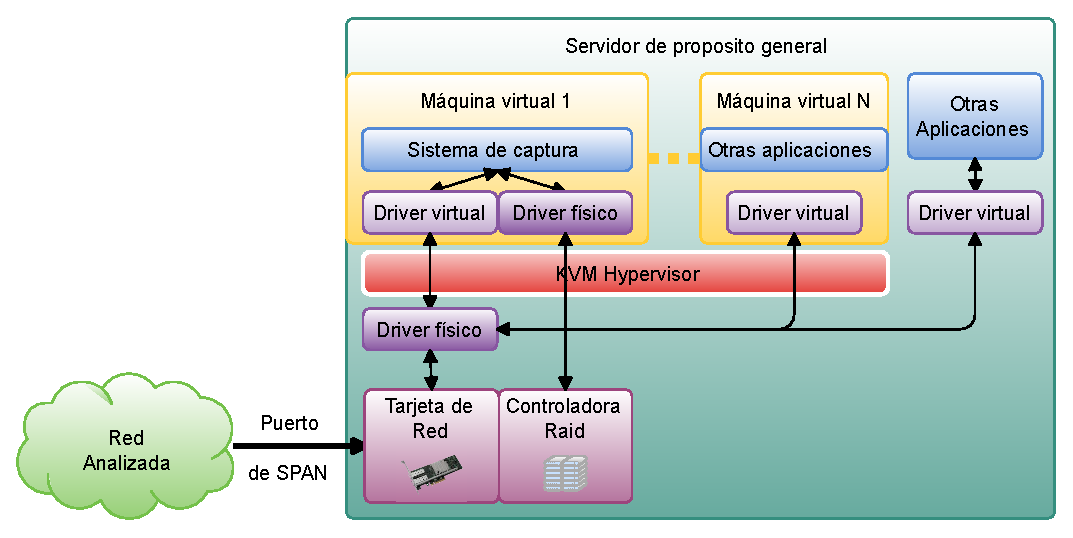
\includegraphics[scale=.7]{VMsriov}
\caption{Arquitectura de captura en un escenario con SRIOV y NFVs}
\label{fig:vmsriov} 
\end{figure}

%contar la diferencia de generación de NFV
\subsubsection{Comparativa de construcción de \glspl{nfv}}

Para que un dispositivo genere funciones virtuales, es necesaria la presencia de un driver en la máquina anfitriona que configure el dispositivo físico (número de \glspl{vf}, tamaños de las colas, reparto de interrupciones, etc). Para el caso de las tarjetas de Intel de 10~Gbps, el driver \gls{vanilla} ofrece esta funcionalidad de una manera muy cómoda. Este driver cumple con la filosofía de \gls{sriov} de delegar en la tarjeta todo el proceso de reparto de interrupciones y paquetes entre las diferentes \gls{nfv}.

No obstante, Intel ofrece una segunda forma de gestionar estas \glspl{nfv}. Los drivers de \gls{dpdk} permiten a su vez generar estas funciones virtuales, pero a diferencia del driver \textit{ixgbe}, es necesario ejecutar un programa sobre \gls{dpdk} para que estas \gls{nfv} reciban tráfico. El programa, conocido como \textit{testpmd}, ayuda activamente a la tarjeta liberándola en parte de la lógica que supone realizar de switch y la copia de paquetes entre la cola de recepción física y las colas asociadas a cada función virtual.
A su vez este programa permite configurar elementos a muy bajo nivel de la tarjeta, que en el driver \textit{ixgbe} supondría modificar el código del propio driver.

En la tabla~\ref{tab:vmsriov:sriov} se muestra una comparativa entre los diferentes métodos de generación de \gls{nfv}. Claramente, parece que el sistema de generación mediante \gls{dpdk} supera por mucho en rendimiento al driver \gls{vanilla}. Por otro lado, para que la aplicación \textit{testpmd} funcione a pleno rendimiento, es necesario reservarla un \gls{core} completo por cada función virtual, al igual que otro \gls{core} para ejecutar la interfaz. Esta limitación obliga a la larga a disponer de un gran número de cores que tan solo copian paquetes entre colas físicas y virtuales.

\begin{table}[htb]
\centering
\begin{tabular}{|c|c|c|}
	\hline
		\multirow{2}{*}{\begin{tabular}[c]{c}{\bf Motor}\\ {\bf de captura}\end{tabular}} & \multicolumn{2}{c|}{{\bf \% de paquetes procesados}}\\
	\cline{2-3}
		 & {\bf Gen. Ixgbe }   & {\bf Gen. \gls{dpdk}}    \\ \hline
		ixgbevf         & >0.1  & 1     \\ \hline
		HPCAPvf         & 36.2  & 82.7     \\ \hline
		DPDK            & 37.6  & 100    \\ \hline
\end{tabular}
\caption{Porcentaje de paquetes capturados en función del método de generación de NFV. El tráfico utilizado estaba formado por paquetes de tamaño mínimo (64Bytes).}
\label{tab:vmsriov:sriov}
\end{table}


\subsubsection{Pruebas de recepción con \glspl{nfv}}

De cara a realizar pruebas con \glspl{nfv}, es necesario mencionar algunos detalles implementativos. Cada \gls{nfv}, a diferencia de su hermana física, tiene una única cola de recepción y transmisión. Por temas de diseño, las \glspl{nfv} tampoco cuentan con contadores de paquetes perdidos, o erróneos, por lo que obtener estos datos es necesario inferirlos de las estadísticas que ofrecen las funciones físicas. Por este motivo, no se han podido medir con exactitud las pérdidas en los diferentes escenarios con \gls{nfv}, no obstante, se han obtenido datos bastante aproximados.

Como se ha mencionado anteriormente, la tarjeta física, es la encargada en última instancia de gestionar hacia que \gls{nfv} se envía cada uno de los paquetes recibidos. Para determinarlo, cada \gls{nfv} posee su propia dirección MAC virtual. Con el objetivo de probar la escalabilidad en función de máquinas virtuales y \glspl{nfv} por \gls{nic} física, se han utilizado 3 máquinas virtuales con dos 2 \glspl{core} virtuales cada una.
Cada \gls{vm} cuenta con una \gls{nfv} con MAC única. Para medir el rendimiento, estas máquinas virtuales ejecutan en paralelo la versión de solo captura desarrollada en \gls{dpdk}. Para realizar las pruebas se han creado 3 trazas de tráfico sinténtico. La primera traza contiene paquetes de tamaño 64 Bytes, todos ellos con una única dirección MAC. La segunda traza, contiene 2 direcciones MAC en una proporcion del 50\% cada una. La tercera traza, contiene 3 direcciones MAC, en una proporcion del 33.3\% cada una.

Los resultados obtenidos de las pruebas figura en la tabla~\ref{tab:vmsriov:rnfv}. En esta tabla, se pueden observar ligeras pérdidas pues no se llegan a alcanzar los 10~Gbps. No obstante, el rendimiento parece escalar y no se ve aparentemente afecto por el número de \glspl{nfv} que hay en el sistema o el número de máquinas virtuales en ejecución.

\begin{table}[htb]
\centering
\begin{tabular}{|c|c|c|}
	\hline
		\multirow{2}{*}{\begin{tabular}[c]{c}{\bf Número de}\\ {\bf MACs emitidas}\end{tabular}} & \multicolumn{2}{c|}{{\bf \% de paquetes procesados}}\\
	\cline{2-3}
		 & {\bf Por cada \gls{vm} }   & {\bf En total}    \\ \hline
		1         & 99.5  & 99.5     \\ \hline
		2         & 49.7  & 99.4     \\ \hline
		3         & 33.2  & 99.5     \\ \hline
\end{tabular}
\caption{Porcentaje de paquetes capturados en función del número de \glspl{vm} y de direcciones MAC destino}
\label{tab:vmsriov:rnfv}
\end{table}

\subsubsection{\glspl{nfv} con captura promíscua}

No obstante, el método nativo de funcionamiento de las \gls{nfv}, no nos sirve para poder construir una sonda de tráfico virtual, pues en un principio solo seríamos capaces de capturar el tráfico destinado a nuestra función virtual. Si el objetivo de nuestro sistema es ofrecer un servicio por una determinada interfaz y a la vez capturar por esta, podemos recurrir a la bandera \gls{mpe}~\cite{825992010}. Esta bandera puede ser configurada a través del programa \textit{testpmd}, e indica a la tarjeta que reenvíe todos aquellos paquetes sin destino conocido a una determinada \gls{nfv}. Nótese, que esta aproximación no nos reenvía aquellos paquetes destinados a una dirección MAC asociada a otra \gls{nfv} de nuestro sistema. No obstante, esta aproximación es sencilla y permite a la tarjeta funcionar a alta velocidad, además de ser completamente válida si mantenemos la arquitectura del típico puerto de SPAN.

En la tabla~\ref{tab:vmvirtio:soloCapA} se muestran los resultados de solo captura. En este escenario, se pretende probar el rendimiento que ofrecen las \glspl{nfv} bajo condiciones habituales. Para ello, se realizan 3 pruebas simples: Una única \gls{vm} conectada a una \gls{nfv}, una única \gls{vm} conectada a dos \gls{nfv} (cada una correspondiente a una \gls{nic} diferente) y finalmente, 2 \glspl{vm} conectadas a 2 \gls{nfv} generadas a partir de la misma \gls{nic}.
%
Los resultados de la tabla son en parte similares a otras pruebas ya realizadas, aunque caben destacar algunos resultados. Para el caso de \textit{HPCAPfv}, al gestionar 2 \glspl{nfv} en una máquina virtual con pocos recursos, se ve saturado rápidamente y el rendimiento cae por falta de \glspl{core}. En el caso de utilizar dos máquinas virtuales en paralelo compartiendo \gls{nic}, se observa que tanto en el motor \gls{dpdk} como en el motor de captura\textit{HPCAPvf}, tienen resultados similares. Esta última prueba de doble \gls{nfv} y doble \gls{vm}, se realizó mediante una traza de paquete mínimo con la MAC destino a broadcast, de forma que todos las \glspl{nfv} recibieran todos y cada uno de los paquetes. Si tenemos esto en cuenta, aunque el tráfico que llega por la interfaz se recibe a 10~Gbps, la tarjeta debe enviar datos a las diferentes \glspl{nfv} a 20~Gbps. Con esto en mente, el 51\% o el 44.1\% de 20~Gbps, se asemeja mucho a valores obtenidos anteriormente.

\begin{table}[htb]
\centering
\begin{tabular}{|c|c|c|c|c|c|c|}
	\hline
		\multirow{3}{*}{\begin{tabular}[c]{c}{\bf Motor}\\ {\bf de captura}\end{tabular}} & \multicolumn{6}{c|}{{\bf \% de paquetes procesados}}\\
	\cline{2-7}
		 & \multicolumn{2}{c|}{{\bf 1 \gls{nfv}}} & \multicolumn{2}{c|}{{\bf 2 \glspl{nfv}}} & \multicolumn{2}{c|}{{\bf (1+1) 2\glspl{nfv}/2\glspl{vm}}} \\
	\cline{2-7}
		 & {\bf 64 Bytes }   & {\bf CAIDA}  & {\bf 64 Bytes}   & {\bf CAIDA} & {\bf 64 Bytes}   & {\bf CAIDA}  \\ \hline
		ixgbePvf      & 1     & 34.2    & 1     & 42.4     & 0.9   & 14.8    \\ \hline
		HPCAPvf       & 82.7  & 100     & 13.0  & 100      & 44.1  & 82.7    \\ \hline
		DPDK          & 100   & 100     & 100   & 100      & 50.8  & 83.0    \\ \hline
\end{tabular}
\caption{Porcentaje de paquetes capturados y no almacenados en un escenario con SRIOV y flag MPE.}
\label{tab:vmvirtio:soloCapA}
\end{table}

%%%%
En la tabla~\ref{tab:vmvirtio:CapAlmac1} se muestran los resultados de captura y almacenamiento cuando solo hay una única \gls{nfv} y una única \gls{vm} en ejecución. Es interesante apreciar como la sobrecarga de la virtualización con \gls{virtio} y \gls{nfv} incrementa lo suficiente la latencia del pipeline de captura de la herramienta de \gls{dpdk} como para hacerla perder una enorme cantidad de paquetes.

\begin{table}[htb]
\centering
\begin{tabular}{|c|c|c|c|c|}
	\hline
		\multirow{3}{*}{\begin{tabular}[c]{c}{\bf Motor}\\ {\bf de captura}\end{tabular}} & \multicolumn{4}{c|}{{\bf \% de paquetes procesados}}\\
	\cline{2-5}
		 & \multicolumn{2}{c|}{{\bf Raid en Passthrough}} & \multicolumn{2}{c|}{{\bf Raid en VirtIO}} \\
	\cline{2-5}
		 & {\bf 64 Bytes }   & {\bf CAIDA}  & {\bf 64 Bytes}   & {\bf CAIDA}  \\ \hline
		HPCAPvf       & 82.6  & 100    & 82.3    & 100     \\ \hline
		DPDK          & 94.2  & 100    & 68.2    & 100  \\ \hline
\end{tabular}
\caption{Porcentaje de paquetes almacenados en un escenario con SRIOV y flag MPE.}
\label{tab:vmvirtio:CapAlmac1}
\end{table}

\subsubsection{\glspl{nfv} con captura global}

En las secciones anteriores de \glspl{nfv}, se ha hablado acerca de como funciona el reparto de paquetes entre las diferentes funciones y de como es posible capturar tráfico que no va destinado a ninguna función virtual. No obstante, uno de los objetivos de este trabajo es evaluar el proceso de monitorización en redes virtuales. Para lograrlo, el datasheet de las tarjetas de Intel~\cite{825992010} nos proporciona información acerca del concepto de \textit{Port Mirroring}. A través de una serie de registros, es posible indicar a la tarjeta de red, que copie todos los paquetes que entren o salgan de una cola a otra cola. Dado que cada \gls{nfv}, tiene asociada una única cola, es posible forzar la copia del contenido de una \gls{nfv} a otra \gls{nfv}. Toda esta configuración de \textit{mirroring} puede ser configurada a través de la aplicación \textit{testpmd}.

La idea principal para realizar esta prueba consiste en utilizar las 3 máquinas virtuales mencionadas al inicio de esta subsección como consumidoras de tráfico, mientras que una cuarta máquina virtual, con la configuración estándar utilizada hasta ahora(y descrita en la sección~\ref{sec:sw}), monitorice el tráfico entre dichas \glspl{vm}.
Dado que el equipo de pruebas tiene arquitectura \gls{numa} y los recursos de las 4 \glspl{vm} exceden los recursos de un procesador, es necesario distribuir las diferentes \glspl{vm} entre los procesadores. Dado que la localización de las \gls{vm} puede afectar al rendimiento, se ha decidido agrupar las 3 \glspl{vm} consumidoras en un mismo procesador, pues comparten funcionalidad similar, y la \gls{vm} de monitorización en otro procesador. 

En la tabla~\ref{tab:vmvirtio:CapAlmac2} se muestra un breve resumen de las pruebas realizadas. Por un lado, los resultados muestran una tasa acotada de Gbps que pueden ser capturados mediante este método. Dado que el \textit{Port Mirroring} consiste en duplicar todos y cada uno de los paquetes, el hecho de que el rendimiento decrezca es razonable, pues en definitiva se están recibiendo al menos el doble Gbps.
Un dato curioso, son los resultados de rendimiento. Si recordamos la arquitectura de la sonda de prueba, el tarjeta de red se encuentra conectada en el nodo \gls{numa}. Dado que este nodo es el más cercano a la tarjeta, parece razonable ejecutar la \gls{vm} en este nodo. No obstante, cuando la \gls{vm} es capaz de capturar mucho más tráfico cuando se encuentra en el nodo \gls{numa} 1.
Este efecto ha de tenerse en cuenta, pues el \textit{Port Mirroring}, no redirige los paquetes a la \gls{vm} de captura, salvo que dicho paquete ya haya sido atendido por la \gls{vm} adecuada. Por ello, situar las máquinas consumidoras en el nodo más cercano a la tarjeta favorece la cantidad de paquetes capturados mediante la técnica del \textit{Port Mirroring}.

\begin{table}[!htb]
\centering
\begin{tabular}{|c|c|c|c|}
	\hline
	\multirow{2}{*}{\begin{tabular}[b]{c}{\bf Motor}\\ {\bf de captura}\end{tabular}} & \multirow{2}{*}{\begin{tabular}[b]{c}{\bf Nodo Numa}\\ {\bf de captura}\end{tabular}} & \multicolumn{2}{c|}{{\bf \% de paquetes procesados}}\\
	\cline{3-4}
	& &  {\bf 64 Bytes } & {\bf CAIDA} \\
	\hline
			\multirow{2}{*}{HPCAPvf} & 0  &  30.7   &  48.0  \\
		\cline{2-4} 
			& 1  &   47.4  &  76.7  \\
	\hline
			\multirow{2}{*}{DPDK} & 0  &  22.8   & 38.4   \\
		\cline{2-4} 
			& 1  &   50.4  &  76.8  \\
	\hline
\end{tabular}
	\caption{Porcentaje de paquetes almacenados en un escenario con SRIOV y Port Mirroring. Captura del tráfico interno de una red virtual formada por 3 VMs. El raid de almacenamiento se encuentra configurado con VirtIO}
	\label{tab:vmvirtio:CapAlmac2}
\end{table}
